\documentclass{beamer}
\beamertemplatenavigationsymbolsempty
\usecolortheme{beaver}
\setbeamertemplate{blocks}[rounded=true, shadow=true]
\setbeamertemplate{footline}[page number]
%
\usepackage[utf8]{inputenc}
\usepackage[english]{babel}
\usepackage{amssymb,amsfonts,amsmath,mathtext}
\usepackage{subfig}
\usepackage[all]{xy} % xy package for diagrams
\usepackage{array}
\usepackage{comment}
\usepackage{multicol}% many columns in slide
\usepackage{hyperref}% urls
\usepackage{hhline}%tables
% Your figures are here:
\graphicspath{ {fig/} {../fig/} }

%----------------------------------------------------------------------------------------------------------
\begin{comment}
\title[\hbox to 56mm{Feature generation}]{Feature generation for classification and forecasting problems}
\author[N.\,P.~Ivkin]{Nikita Ivkin}
\institute{Moscow Institute of Physics and Technology}
\date{\footnotesize
\par\smallskip\emph{Course:} My first scientific paper\par (Strijov's practice)/Group 874 %821, 813
\par\smallskip\emph{Expert:} I.\,F.~Anny
\par\smallskip\emph{Consultant:} I.\,O.~Gordeos
\par\bigskip\small 2021}
\end{comment}
%----------------------------------------------------------------------------------------------------------
\begin{document}
%----------------------------------------------------------------------------------------------------------
%\begin{frame}
%\thispagestyle{empty}
%\maketitle
%\end{frame}
%-----------------------------------------------------------------------------------------------------
%\begin{frame}{Goal of research}
%..
%\end{frame}
%-----------------------------------------------------------------------------------------------------
\begin{frame}{One-slide talk}
\begin{figure}[h]
{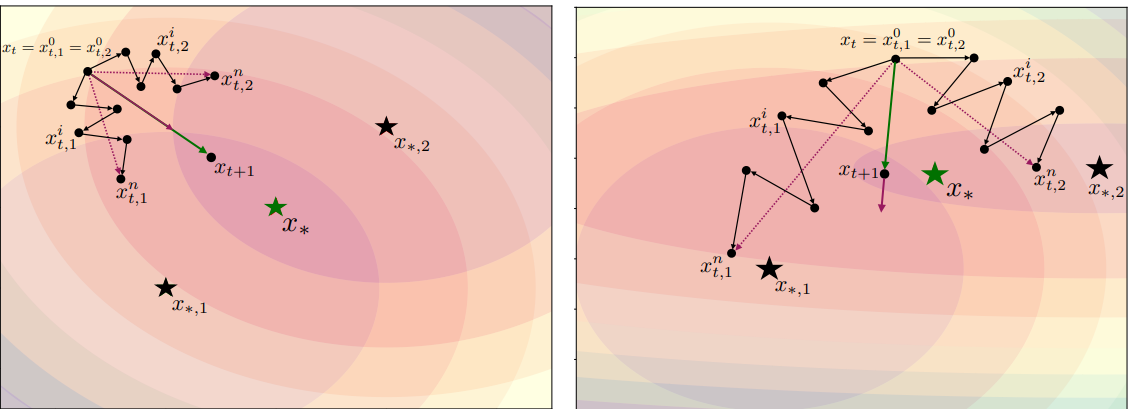
\includegraphics[scale=0.18]{figures/ServerStep.png} \\ Server Step-Sizes}
\end{figure}

\begin{columns}[c]
\column{0.6\textwidth}
%\includegraphics[width=1.0\textwidth]{ErrorFunction}
    \begin{figure}[h]
    \center{\includegraphics[scale=0.3]{figures/Distributed methods.png} \\ Distributed methods comparison}
\end{figure}
\column{0.5\textwidth}
    We will be combining techniques to improve performance
\end{columns}

\end{frame}


%----------------------------------------------------------------------------------------------------------
%\begin{frame}{Problem statement}
%.
%\end{frame}
%----------------------------------------------------------------------------------------------------------
\begin{comment}

\begin{frame}{Solution}

\begin{columns}[c]
\column{0.6\textwidth}
    Column 1
\column{0.4\textwidth}
    Column 2
\end{columns}
\end{frame}

\end{comment}
%----------------------------------------------------------------------------------------------------------
%\begin{frame}{Computational experiment}
%..
%\end{frame}
%----------------------------------------------------------------------------------------------------------
\begin{comment}
\begin{frame}{Conclusion}
    \begin{block}{Forecast with hierarchical aggregation of}
    \begin{itemize}
        \item types of freight in
        \item stations, regions, and roads,
        \item for a day, week, month, and quarter.
    \end{itemize}
    \end{block}
\end{frame}
\end{comment}
%----------------------------------------------------------------------------------------------------------
\end{document} 
